\section{DMD Analysis}
\label{ch:dmd}

Open from `3.\ Analysis $\to$ DMD Analysis`.

```{note}
DMD requires \textbf{time-resolved} data and at least 50 snapshots. The button is greyed out for non-TR datasets.
```

Dynamic Mode Decomposition (DMD) extracts spatial modes that oscillate at a single frequency and grow or decay at a single rate. Unlike POD, DMD modes are not ordered by energy but by their dynamic content. This makes DMD ideal for isolating periodic phenomena such as vortex shedding, acoustic resonances, or shear layer flapping (Schmid, 2010; Tu et al., 2014).

\noindent\textbf{References:} Schmid, P.J. (2010). Dynamic mode decomposition of numerical and experimental data. \textit{Journal of Fluid Mechanics}, 656, 5--28. Tu, J.H., Rowley, C.W., Luchtenburg, D.M., Brunton, S.L. \& Kutz, J.N. (2014). On dynamic mode decomposition: theory and applications. \textit{Journal of Computational Dynamics}, 1(2), 391--421.

\subsection{Computing DMD}

```{note}
\begin{enumerate}[leftmargin=1.5em, topsep=2pt]
  \item Set `Rank truncation` (default 50). This caps the number of DMD modes.
  \item Optionally enable a Strouhal number normalization with a reference length and velocity.
  \item Click `Compute DMD`.
\end{enumerate}
```

\subsection{Spectrum tab}

The spectrum shows each DMD mode as a bubble in the frequency-growth-rate plane, with bubble area proportional to mode amplitude. Click on any bubble to display its spatial structure in the Mode tab. A growth-rate filter $|\sigma| < $ threshold can be applied to focus on near-neutral physically meaningful modes.

\subsection{Mode tab}

Displays the spatial structure (real and imaginary parts) of the currently selected DMD mode for the chosen velocity component.

\begin{figure}[htbp]
  \centering
  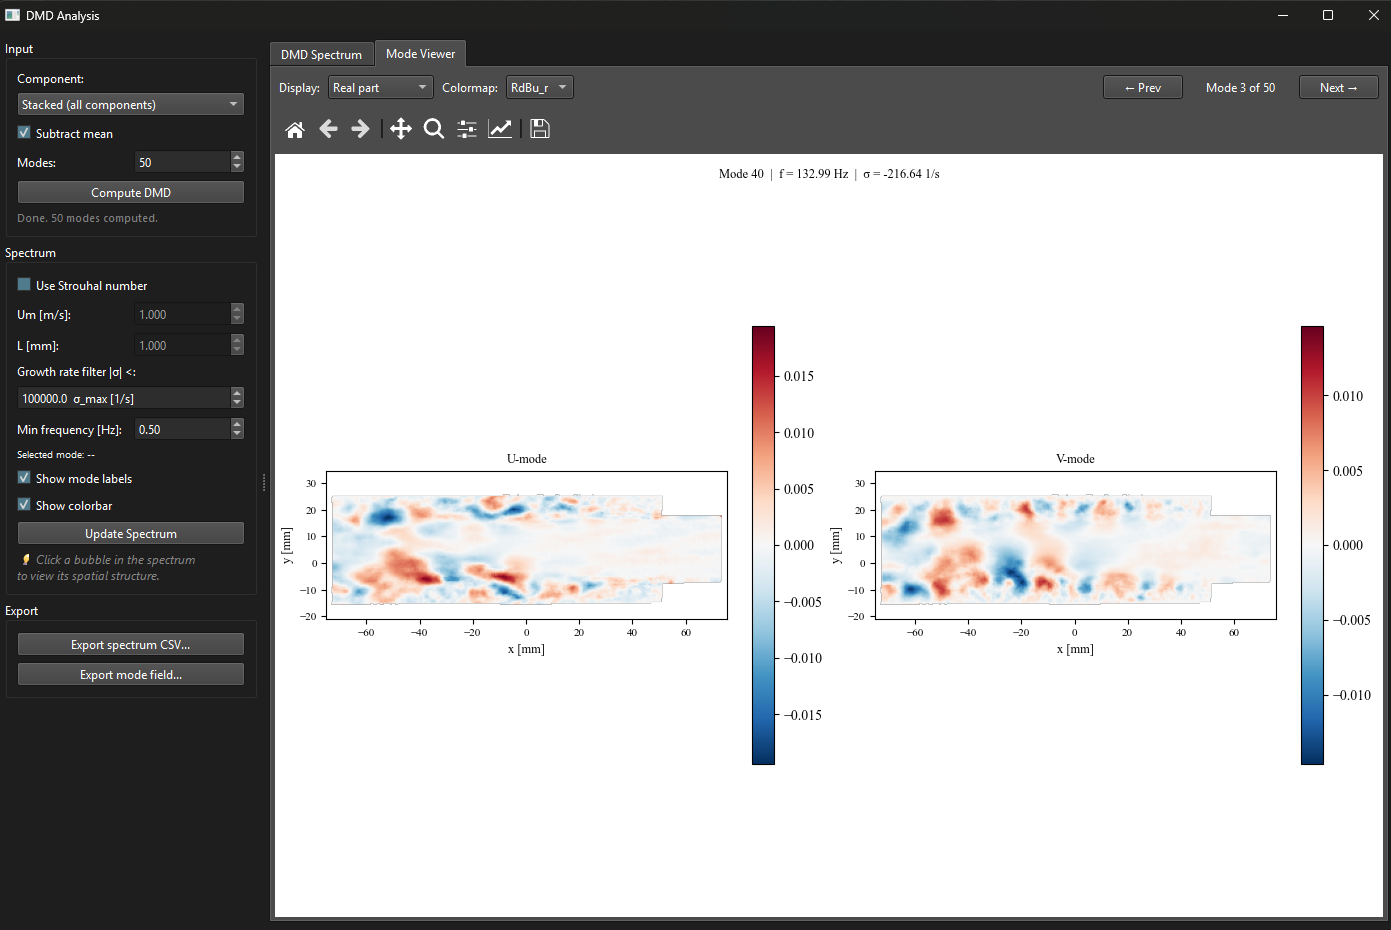
\includegraphics[width=0.92\linewidth]{fig_dmd_mode}
  \caption{DMD Mode tab showing the real and imaginary parts of a selected mode. Animating between them gives a sense of the structure's oscillation in time.}
  \label{fig:dmd_mode}
\end{figure}

```{tip}
The real and imaginary parts of a DMD mode represent the two phases of the oscillation separated by a quarter period. Animating between them (real $\to$ imaginary $\to$ $-$real $\to$ $-$imaginary) gives a physical sense of how the structure evolves in time.
```

\subsection{Exporting}

Click `Export spectrum CSV\ldots` to save a table of all modes with their frequency, growth rate, and amplitude. Click `Export mode field\ldots` to save the spatial structure of the currently selected mode as a Tecplot \texttt{.dat} file.

% ============================= CHAPTER 12 ==============================
